\documentclass{article}
\usepackage{polski}
\usepackage{graphicx}
\usepackage{titling}
\usepackage{tabularx} % in the preamble
\usepackage{hyperref}


\usepackage[utf8]{inputenc}


\title{Wiosenna szkoła brydża dla początkujących}
\date{}
\author{}


\usepackage{tikz}    
\setlength{\droptitle}{-8em}   % This is your set screw

\begin{document}
\maketitle
\vspace{-50px}
\begin{itemize}
	\item Chcesz poprawić swoją koncentrację i zdolności analityczne?
	\item Zależy Ci na poznaniu nowej, fascynującej gry z bogatą historią?
	\item Masz już doświadczenie i chcesz zgłębić tajniki gry?
	\item A może chcesz spędzić miło czas wśród ciekawych osób dzielących tę samą pasję?
\end{itemize}
\begin{tikzpicture}[remember picture,overlay]
   \node[anchor=north east,inner sep=0pt] at (current page.north east)
              {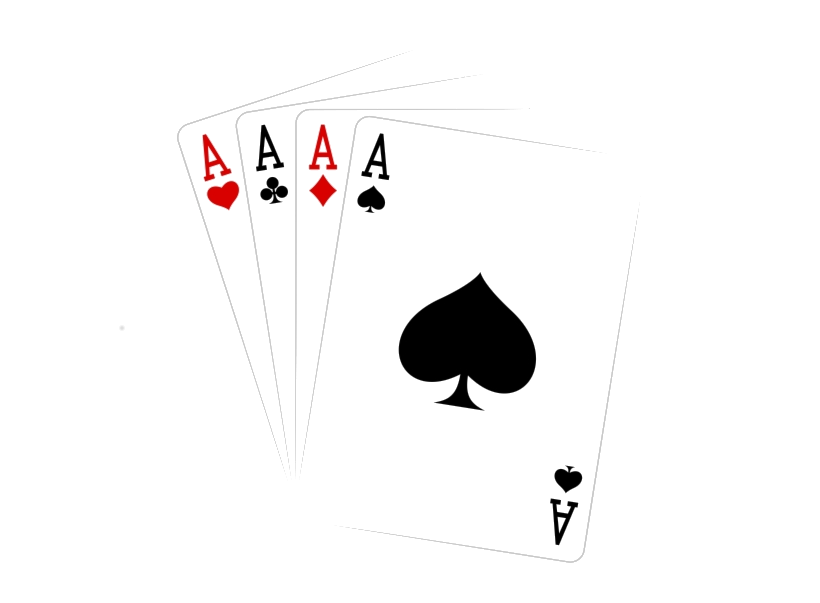
\includegraphics[scale=0.2]{aces2.png}};
\end{tikzpicture}
Zapraszam na wiosenną szkołę brydża dla młodszych i starszych, która rusza 21 marca na Ochocie i pozwoli Wam nauczyć się podstaw brydża sportowego.
Podczas 5 tygodni kursu poznasz brydżowe podstawy, techniki licytacji i ciekawe manewry rozgrywkowe. Dowiesz
się jak skutecznie wistować, a także jak współpracować i wymieniać informacje z partnerem.
Koszt: 299zł.\\\\
Cena zawiera:
\begin{itemize}
	\item Cztery trzygodzinne zajęcia (21 i 28 marca, 4 i 11 kwietnia), na których nauczycie się zasad i znacząco poprawicie poziom swojej gry.
	\item Ostatnie, piąte zajęcia (18 kwietnia) podczas których rozegracie prawdziwy turniej brydżowy.
	\item Internetowy dostęp do profesjonalnych materiałów, które zawierają informacje uzyskane na zajęciach, a także
		problemy sprawdzające i utrwalające zdobytą wiedzę.
	\item Możliwość wypożyczania książek brydżowych z biblioteczki szkoły. Niektórych nie sposób znaleźć gdzie indziej.
	\item Mailowa dostępność trenera, który chętnie odpowie na wszystkie pytania.
\end{itemize}
\vspace{20px}
\centerline{\Large{PROMOCJA}}
\vspace{10px}

Zapisz się do 20 lutego, a otrzymasz 50zł. zniżki. Zabierz ze sobą partnera, a otrzymacie kolejne 50zł. Za cały kurs
zapłacicie wtedy jedyne 199zł.\\\\
\begin{tabularx}{\textwidth}{X r}
	Zapisy i pytania pod numerem: & 794150203\\
	Lub mailowo na adres: & szkola.brydza@gmail.com\\
\end{tabularx}
\end{document}
